\documentclass[a4paper,oneside,DIV=10,12pt]{scrartcl}

\usepackage{float}

\usepackage{fontspec}
\setmainfont{STIX Two Text}
\setsansfont{Roboto}
\setmonofont{PT Mono}

\usepackage{microtype}

\usepackage{amsmath}
\usepackage{unicode-math}
\setmathfont{STIX Two Math}

\usepackage{polyglossia}
\setmainlanguage{ukrainian}

\usepackage{graphicx}

\usepackage{booktabs}
\usepackage{cellspace}
\setlength\cellspacetoplimit{2pt}
\setlength\cellspacebottomlimit{2pt}

\usepackage{subcaption}

\usepackage{siunitx}
\sisetup{output-decimal-marker = {,}}

\newcommand\schel[1]{\textit{#1}}

\begin{document}
	\begin{titlepage}
	\begin{center}
		Міністерство освіти і науки України\\
		Національний авіаційний університет\\
		Навчально-науковий інститут комп'ютерних інформаційних технологій\\
		Кафедра комп'ютеризованих систем управління

		\vspace{\fill}
		Лабораторна робота №4\\
		з дисципліни «Комп'ютерна електроніка»\\
		на тему «Дослідження логічних~елементів»\\
		Варіант №3
		
		\vspace{\fill}
		\begin{flushright}
		Виконав:\\
		студент ННІКІТ СП-225\\
		Клокун Владислав\\
		Перевірив:\\
		Андрєєв О. В.
		\end{flushright}
		
		Київ 2017
	\end{center}
	\end{titlepage}
	
	\section{Мета та основні завдання роботи}
		\begin{enumerate}
			\item Практична перевірка роботи логічних елементів різних функціонально-повних наборів.
			\item Освоєння методики зняття основних характеристик логічних елементів.
			\item Визначення основних параметрів логічних елементів.
			\item Вивчення законів функціонування логічних елементів «НЕ», «І», «АБО», «АБО—НЕ», «І—НЕ».
			\item Вивчення методики визначення часових параметрів логічних елементів.
		\end{enumerate}
	
	\section{Обладнання та прилади}
		До лабораторної установки входять:
		\begin{enumerate}
			\item Набір логічних елементів «НЕ», «І», «АБО», «АБО—НЕ», «І—НЕ».
			\item Два вольтметра постійної напруги для зняття передавальної характеристики $U_{\text{ВИХ}} = f \left(U_{\text{ВХ}}\right)$.
			\item Двопроменевий осцилограф.
			\item Набір схем для дослідження логічних елементів в статичному і динамічному режимах.
		\end{enumerate}
		
	\section{Хід роботи}
		\subsection{Дослідження логічного елемента «НЕ»}
			Готуємо віртуальну лабораторну установку до роботи. Для цього встановлюємо такі параметри:
			\begin{table}[!htbp]
			\centering
				\begin{tabular}{lccr}
				Time Base & 0{,}5~s  &                     & Y/T, Auto\\
				Channel A & 10~V/div & Y position: 0{,}00  & DC\\
				Channel B & 10~V/div & Y position: −2{,}20 & DC\\
				\end{tabular}
			\end{table}
			
			Вимірюємо часові параметри логічного елемента «НЕ». Для цього вмикаємо лабораторну установку на моделювання. Лабораторна установка зображена на рисунку~\ref{fig:NOT-schematic}. Результати вимірювань наведені у таблиці~\ref{tab:NOT-time-params}.
			
			\begin{figure}
			\centering
				\begin{subfigure}[b]{0.5\textwidth}
				\centering
					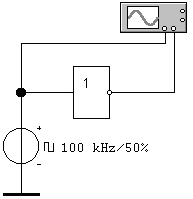
\includegraphics[]{schematics/01-01-not.png}
				\caption{Принципова схема для вимірювання часових параметрів елемента «НЕ»}
				\label{fig:NOT-schematic}
				\end{subfigure}
				~
				\begin{subtable}[b]{0.4\textwidth}
				\centering
					\begin{tabular}{ClCr}
						\toprule
							Параметр & Значення \\
						\midrule
							$t^{01}$                & \SI{27,5}{\nano\second}\\
							$t^{01}_{\text{ЗТ}}$    & \SI{ 279}{\nano\second}\\
							$t^{01}_{\text{ЗТ.Р}}$  & \SI{ 420}{\nano\second}\\
							$t^{10}$                & \SI{  27}{\nano\second}\\
							$t^{10}_{\text{ЗТ}}$    & \SI{  20}{\nano\second}\\
							$t^{10}_{\text{ЗТ.Р}}$  & \SI{26,5}{\nano\second}\\
						\bottomrule
					\end{tabular}
				\caption{Часові параметри логічного елемента «НЕ»}
				\label{tab:NOT-time-params}
				\end{subtable}
			\caption{Вимірювання часових параметрів логічного елемента «НЕ»}
			\end{figure}
			
			Будуємо передавальну характеристику $U_2 = f(U_1)$ елемента «НЕ». Для цього встановлюємо вхідну напругу рівною \SI{0}{\volt} ($U_1 = \SI{0}{\volt}$). Встановлюємо опір потенціометра $R = 0\%$. Потім покроково збільшуємо опір (кожен крок — 10\%) та вимірюємо $U_1$ і $U_2$. Схема для побудови передавальної характеристики зображена на рисунку~\ref{fig:NOT-schematic-transfer-params}. Результати наведені у таблиці~\ref{tab:NOT-transfer-params-table}.
			
			\begin{figure}[!htbp]
			\centering
				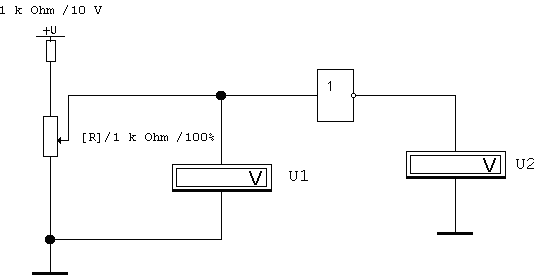
\includegraphics[]{schematics/01-02-not.png}
			\caption{Принципова схема для побудови передавальної характеристики елемента «НЕ»}
			\label{fig:NOT-schematic-transfer-params}
			\end{figure}
			
			\begin{table}[!htbp]
			\centering
				\begin{tabular}{
					l
					S[table-format = 1.3]
					S[table-format = 1.3]
				}
					\toprule
						{$R~(\%)$} & {$U_1~(\si{\volt}$)} & {$U_2~(\si{\volt})$}\\
					\midrule
						0        & 0        & 9,99\\
						10       & 0,597    & 9,99\\
						20       & 1,189    & 9,98\\
						30       & 1,774    & 5,286\\
						40       & 2,349    & 0,136\\
						50       & 2,919    & 0,103\\
						60       & 3,485    & 0,089\\
						70       & 4,050    & 0,081\\
						80       & 4,616    & 0,075\\
						90       & 5,189    & 0,069\\
						100      & 5,758    & 0,066\\
					\bottomrule
				\end{tabular}
			\caption{Передавальна характеристика елемента «НЕ»}
			\label{tab:NOT-transfer-params-table}
			\end{table}
			
			За результатами вимірювань будуємо графік передавальної характеристики $U_2 = f(U_1)$, за яким вимірюємо рівень логічного нуля і логічної одиниці. Графік передавальної характеристики зображений на рисунку~\ref{fig:NOT-transfer-params-plot}.
			
			\begin{figure}[!htbp]
			\centering
				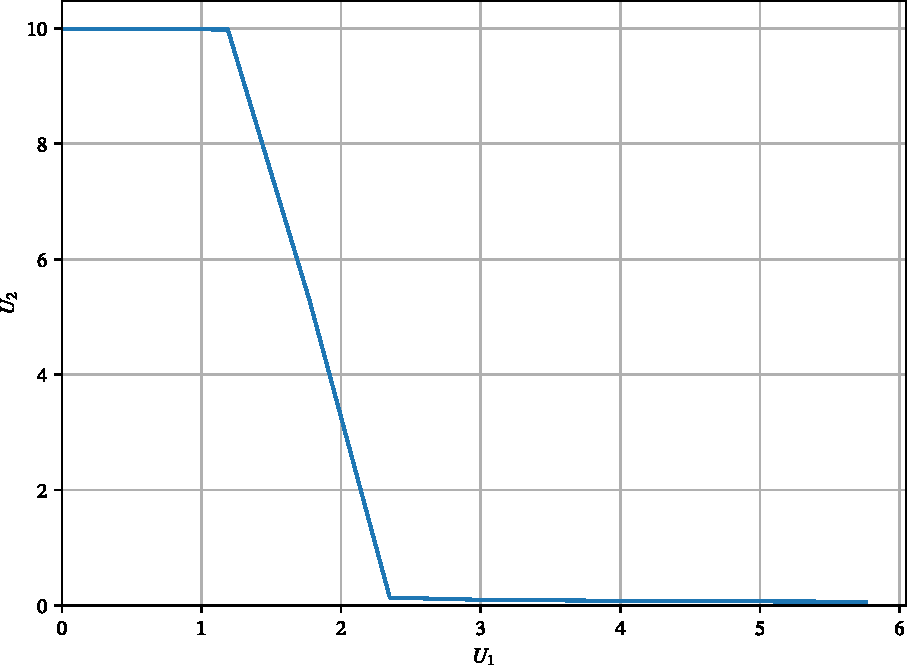
\includegraphics[width=0.9\textwidth]{plots/03-pdf/01-01-not-transfer-params-edited.pdf}
			\caption{Графік передавальної характеристики}
			\label{fig:NOT-transfer-params-plot}
			\end{figure}
			
			Відповідно до таблиці істинності перевіряємо закон функціонування логічного елемента «НЕ» за допомогою індикаторів рівня, вольтметра і схеми, зображеної  на рисунку~\ref{fig:NOT-functioning-law-schematic}.
			
			\begin{figure}[!htbp]
			\centering
				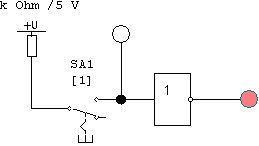
\includegraphics[]{schematics/01-03-not.png}
			\caption{Принципова схема для перевірки закону функціонування елемента «НЕ»}
			\label{fig:NOT-functioning-law-schematic}
			\end{figure}
			
			Будуємо таблицю істинності для логічного елемента «НЕ», в якій замість «0» і «1» наведені відповідні потенціали. Результати наведені в таблиці~\ref{tab:not-truth-table}.
			
			\begin{table}[!htbp]
			\centering
				\begin{tabular}{lr}
					\toprule
						$x_1$ & $f(x)$\\
					\midrule
						\SI{1,189}{\volt} & \SI{9,980}{\volt}\\
						\SI{2,349}{\volt} & \SI{0,136}{\volt}\\
					\bottomrule
				\end{tabular}
			\caption{Таблиця істинності логічного елемента «НЕ»}
			\label{tab:not-truth-table}
			\end{table}
			
			Перевіряємо динамічний режим роботи елемента «НЕ» за допомогою схеми, зображеної на рисунку~\ref{fig:schematic-not-dynamic-mode}.
			
			\begin{figure}[!htbp]
			\centering
				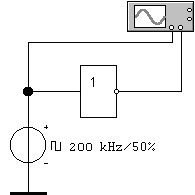
\includegraphics[]{schematics/01-04-not.png}
			\caption{Принципова схема для перевірки динамічного режиму роботи елемента «НЕ»}
			\label{fig:schematic-not-dynamic-mode}
			\end{figure}
			
			За результатами перевірки будуємо часову діаграму елемента «НЕ». Побудована діаграма зображена на рисунку~\ref{fig:not-time-diagram}.
			
			\begin{figure}[!htbp]
			\centering
				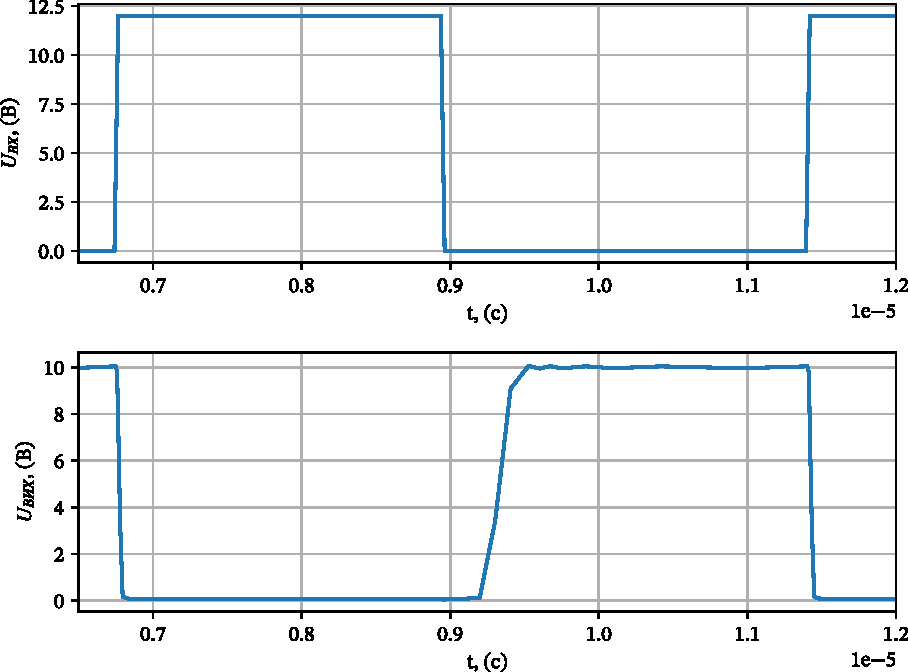
\includegraphics[width=\textwidth]{plots/03-pdf/01-NOT-time-diagram-edited.pdf}
			\caption{Часова діаграма логічного елемента «НЕ»}
			\label{fig:not-time-diagram}
			\end{figure}
			
		\subsection{Дослідження логічного елемента «І»}
			Перевіряємо закон функціонування логічного елемента «І» за допомогою індикаторів рівня вхідних сигналів $x_1$ і $x_2$, які комутуються перемикачами \schel{SA1} і \schel{SA2}. Схема для дослідження зображена на рисунку~\ref{fig:AND-function-law-schematic}.
		
			\begin{figure}[!htbp]
			\centering
				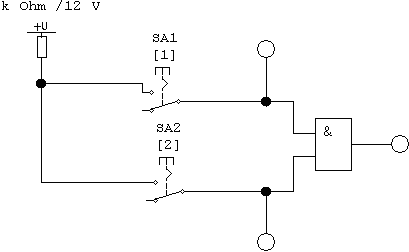
\includegraphics[]{schematics/02-01-AND.png}
			\caption{Принципова схема для перевірки закону функціонування логічного елемента «І»}
			\label{fig:AND-function-law-schematic}
			\end{figure}
			
			Записуємо таблицю істинності, змінюючи значення логічних «0» і «1» на значення відповідних потенціалів. Результати наведені в таблиці~\ref{fig:AND-truth-table-potentials}.
			
			\begin{table}[!htbp]
			\centering
				\begin{tabular}{ccr}
					\toprule
						$x_1$ & $x_2$ & $f(x_1, x_2)$\\
					\midrule
						\SI{1,189}{\volt} & \SI{1,189}{\volt} & \SI{0,136}{\volt}\\
						\SI{1,189}{\volt} & \SI{2,349}{\volt} & \SI{0,136}{\volt}\\
						\SI{2,349}{\volt} & \SI{1,189}{\volt} & \SI{0,136}{\volt}\\
						\SI{2,349}{\volt} & \SI{2,349}{\volt} & \SI{9,980}{\volt}\\
					\bottomrule
				\end{tabular}
			\caption{Таблиця істинності логічного елемента «І» з вказаними потенціалами}
			\label{fig:AND-truth-table-potentials}
			\end{table}
			
			Перевіряємо динамічний режим роботи логічного елемента «І» за допомогою схеми, зображеної на рисунку~\ref{fig:AND-dynamic-mode-schematic}.
			
			\begin{figure}[!htbp]
			\centering
				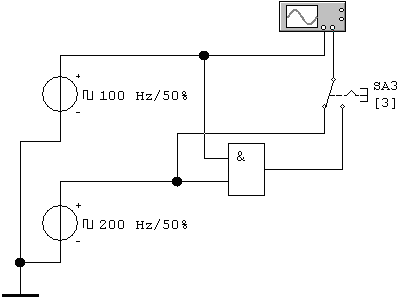
\includegraphics[]{schematics/02-02-AND.png}
			\caption{Принципова схема для перевірки динамічного режиму роботи логічного елемента «І»}
			\label{fig:AND-dynamic-mode-schematic}
			\end{figure}
			
			Отримали осцилограму вхідних сигналів. Встановлюємо перемикач \schel{SA3} у праве положення і отримаємо осцилограму вихідного сигналу.
			
			За отриманими даними будуємо часову діаграму логічного елемента «І». Побудована діаграма зображена на рисунку~\ref{fig:AND-time-diagram}.
			
			\begin{figure}[!htbp]
			\centering
				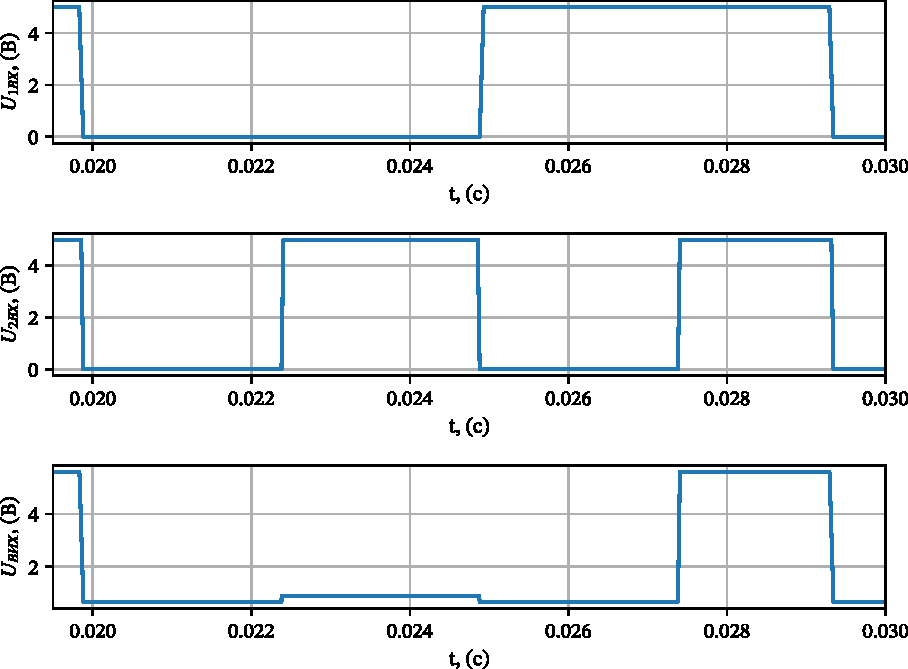
\includegraphics[width=\textwidth]{plots/03-pdf/02-AND-time-diagram-edited.pdf}
			\caption{Часова діаграма логічного елемента «І»}
			\label{fig:AND-time-diagram}
			\end{figure}
			
			За часовою діаграмою по тактах складаємо таблицю істинності логічного елемента «І». Результат наведений у таблиці~\ref{fig:AND-truth-table}.
			
			\begin{table}[!htbp]
			\centering
				\begin{tabular}{ccr}
					\toprule
						$x_1$ & $x_2$ & $f(x_1, x_2)$\\
					\midrule
						0     & 0     & 0\\
						0     & 1     & 0\\
						1     & 0     & 0\\
						1     & 1     & 1\\
					\bottomrule
				\end{tabular}
			\caption{Таблиця істинності логічного елемента «І»}
			\label{fig:AND-truth-table}
			\end{table}
			
		\subsection{Дослідження логічного елемента «АБО»}
			Перевіряємо закон функціонування логічного елемента «АБО» за допомогою індикаторів рівня вхідних сигналів $x_1$ і $x_2$, які комутуються перемикачами \schel{SA1} і \schel{SA2}. Схема для дослідження зображена на рисунку~\ref{fig:OR-function-law-schematic}.
			
			\begin{figure}[!htbp]
			\centering
				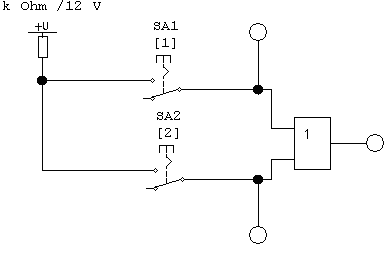
\includegraphics[]{schematics/03-01-OR.png}
			\caption{Принципова схема для перевірки закону функціонування логічного елемента «АБО»}
			\label{fig:OR-function-law-schematic}
			\end{figure}
			
			Записуємо таблицю істинності, змінюючи значення логічних «0» і «1» на значення відповідних потенціалів. Результати наведені в таблиці~\ref{fig:OR-truth-table-potentials}.
			
			\begin{table}[!htbp]
			\centering
				\begin{tabular}{ccr}
					\toprule
						$x_1$ & $x_2$ & $f(x_1, x_2)$\\
					\midrule
						\SI{1,189}{\volt} & \SI{1,189}{\volt} & \SI{0,136}{\volt}\\
						\SI{1,189}{\volt} & \SI{2,349}{\volt} & \SI{9,980}{\volt}\\
						\SI{2,349}{\volt} & \SI{1,189}{\volt} & \SI{9,980}{\volt}\\
						\SI{2,349}{\volt} & \SI{2,349}{\volt} & \SI{9,980}{\volt}\\
					\bottomrule
				\end{tabular}
			\caption{Таблиця істинності логічного елемента «І» з вказаними потенціалами}
			\label{fig:OR-truth-table-potentials}
			\end{table}
			
			Перевіряємо динамічний режим роботи логічного елемента «АБО» за допомогою схеми, зображеної на рисунку~\ref{fig:OR-dynamic-mode-schematic}.
			
			\begin{figure}[!htbp]
			\centering
				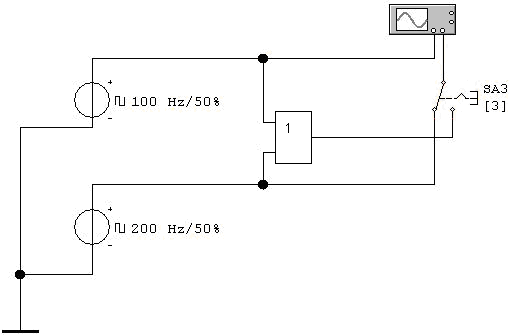
\includegraphics[]{schematics/03-02-OR.png}
			\caption{Принципова схема для перевірки динамічного режиму роботи логічного елемента «АБО»}
			\label{fig:OR-dynamic-mode-schematic}
			\end{figure}
			
			Отримали осцилограму вхідних сигналів. Встановлюємо перемикач \schel{SA3} у праве положення і отримаємо осцилограму вихідного сигналу.
			
			За отриманими даними будуємо часову діаграму логічного елемента «І». Побудована діаграма зображена на рисунку~\ref{fig:OR-time-diagram}.
			
			\begin{figure}[!htbp]
			\centering
				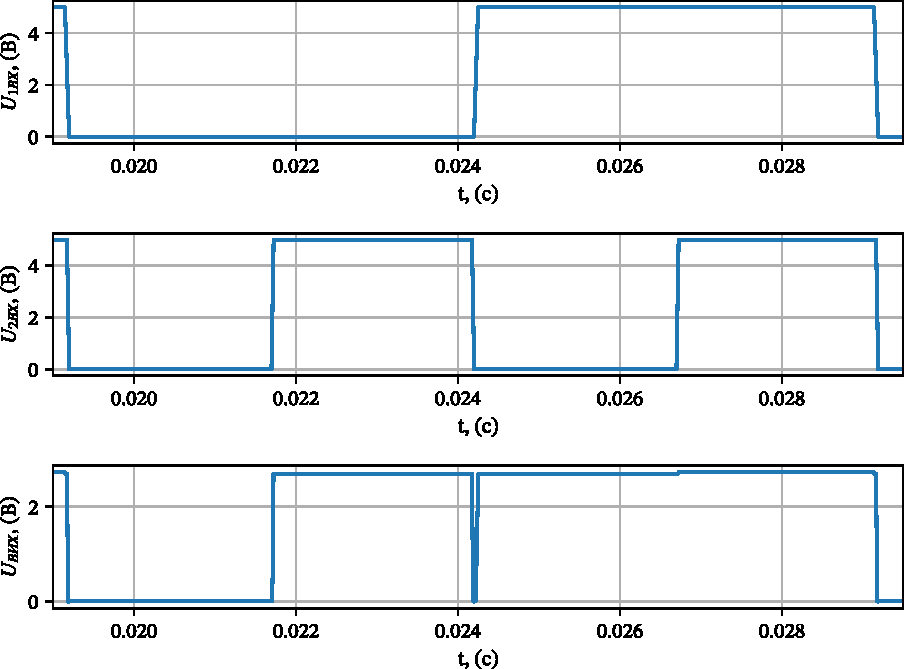
\includegraphics[width=\textwidth]{plots/03-pdf/03-OR-time-diagram-edited.pdf}
			\caption{Часова діаграма логічного елемента «АБО»}
			\label{fig:OR-time-diagram}
			\end{figure}
			
			За часовою діаграмою по тактах складаємо таблицю істинності логічного елемента «АБО». Результат наведений у таблиці~\ref{fig:OR-truth-table}.
			
			\begin{table}[!htbp]
			\centering
				\begin{tabular}{ccr}
					\toprule
						$x_1$ & $x_2$ & $f(x_1, x_2)$\\
					\midrule
						0     & 0     & 0\\
						0     & 1     & 1\\
						1     & 0     & 1\\
						1     & 1     & 1\\
					\bottomrule
				\end{tabular}
			\caption{Таблиця істинності логічного елемента «АБО»}
			\label{fig:OR-truth-table}
			\end{table}
			
		\subsection{Дослідження логічного елемента «І—НЕ»}
			Перевіряємо закон функціонування логічного елемента «І—НЕ» за допомогою індикаторів рівня вхідних сигналів $x_1$ і $x_2$, які комутуються перемикачами \schel{SA1} і \schel{SA2}. Схема для дослідження зображена на рисунку~\ref{fig:NAND-function-law-schematic}.
			
			\begin{figure}[!htbp]
			\centering
				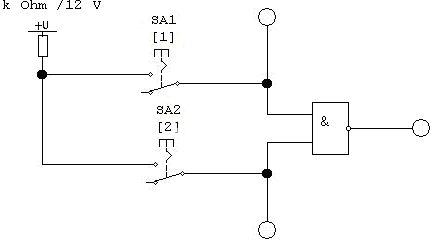
\includegraphics[]{schematics/04-01-NAND.png}
			\caption{Принципова схема для перевірки закону функціонування логічного елемента «І—НЕ»}
			\label{fig:NAND-function-law-schematic}
			\end{figure}
			
			Записуємо таблицю істинності, змінюючи значення логічних «0» і «1» на значення відповідних потенціалів. Результати наведені в таблиці~\ref{fig:NAND-truth-table-potentials}.
			
			\begin{table}[!htbp]
			\centering
				\begin{tabular}{ccr}
					\toprule
						$x_1$ & $x_2$ & $f(x_1, x_2)$\\
					\midrule
						\SI{1,189}{\volt} & \SI{1,189}{\volt} & \SI{9,980}{\volt}\\
						\SI{1,189}{\volt} & \SI{2,349}{\volt} & \SI{9,980}{\volt}\\
						\SI{2,349}{\volt} & \SI{1,189}{\volt} & \SI{9,980}{\volt}\\
						\SI{2,349}{\volt} & \SI{2,349}{\volt} & \SI{0,136}{\volt}\\
					\bottomrule
				\end{tabular}
			\caption{Таблиця істинності логічного елемента «І» з вказаними потенціалами}
			\label{fig:NAND-truth-table-potentials}
			\end{table}
			
			Перевіряємо динамічний режим роботи логічного елемента «І—НЕ» за допомогою схеми, зображеної на рисунку~\ref{fig:NAND-dynamic-mode-schematic}.
			
			\begin{figure}[!htbp]
			\centering
				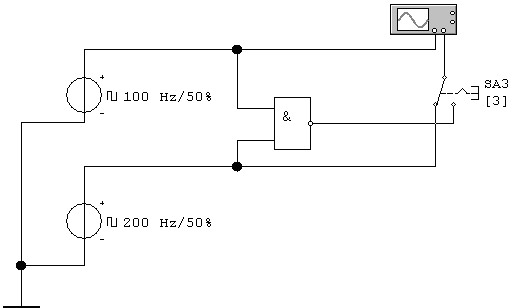
\includegraphics[]{schematics/04-02-NAND.png}
			\caption{Принципова схема для перевірки динамічного режиму роботи логічного елемента «І—НЕ»}
			\label{fig:NAND-dynamic-mode-schematic}
			\end{figure}
			
			Отримали осцилограму вхідних сигналів. Встановлюємо перемикач \schel{SA3} у праве положення і отримаємо осцилограму вихідного сигналу.
			
			За отриманими даними будуємо часову діаграму логічного елемента «І». Побудована діаграма зображена на рисунку~\ref{fig:NAND-time-diagram}.
			
			\begin{figure}[!htbp]
			\centering
				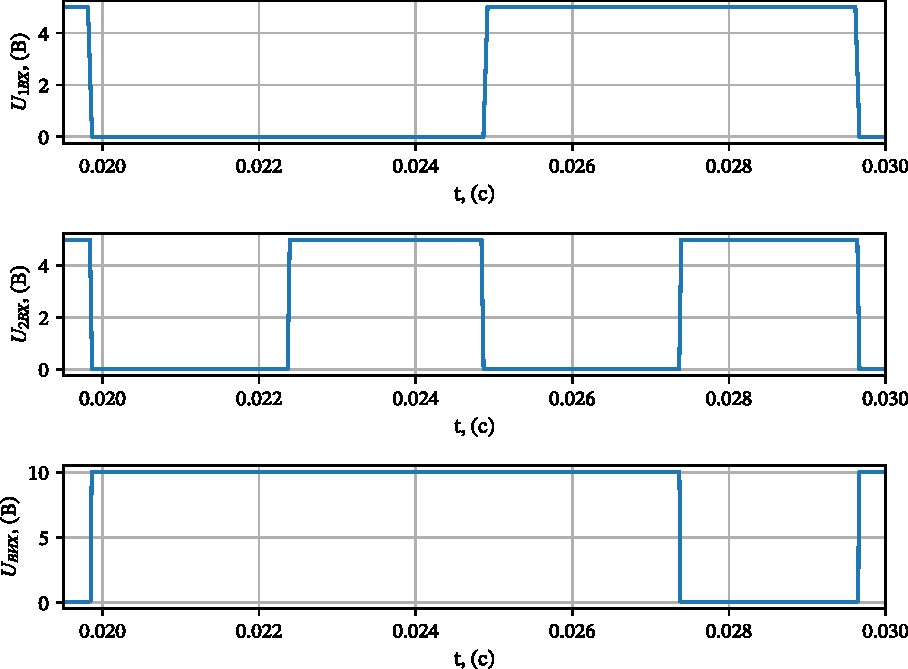
\includegraphics[width=\textwidth]{plots/03-pdf/04-NAND-time-diagram-edited.pdf}
			\caption{Часова діаграма логічного елемента «І—НЕ»}
			\label{fig:NAND-time-diagram}
			\end{figure}
			
			За часовою діаграмою по тактах складаємо таблицю істинності логічного елемента «АБО». Результат наведений у таблиці~\ref{fig:NAND-truth-table}.
			
			\begin{table}[!htbp]
			\centering
				\begin{tabular}{ccr}
					\toprule
						$x_1$ & $x_2$ & $f(x_1, x_2)$\\
					\midrule
						0     & 0     & 1\\
						0     & 1     & 1\\
						1     & 0     & 1\\
						1     & 1     & 0\\
					\bottomrule
				\end{tabular}
			\caption{Таблиця істинності логічного елемента «І—НЕ»}
			\label{fig:NAND-truth-table}
			\end{table}
			
		\subsection{Дослідження логічного елемента «АБО—НЕ»}
			Перевіряємо закон функціонування логічного елемента «АБО—НЕ» за допомогою індикаторів рівня вхідних сигналів $x_1$ і $x_2$, які комутуються перемикачами \schel{SA1} і \schel{SA2}. Схема для дослідження зображена на рисунку~\ref{fig:NOR-function-law-schematic}.
			
			\begin{figure}[!htbp]
			\centering
				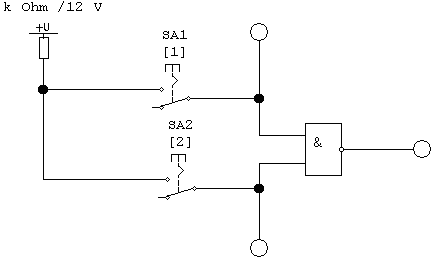
\includegraphics[]{schematics/05-01-NOR.png}
			\caption{Принципова схема для перевірки закону функціонування логічного елемента «АБО—НЕ»}
			\label{fig:NOR-function-law-schematic}
			\end{figure}
			
			Записуємо таблицю істинності, змінюючи значення логічних «0» і «1» на значення відповідних потенціалів. Результати наведені в таблиці~\ref{fig:NAND-truth-table-potentials}.
			
			\begin{table}[!htbp]
			\centering
				\begin{tabular}{ccr}
					\toprule
						$x_1$ & $x_2$ & $f(x_1, x_2)$\\
					\midrule
						\SI{1,189}{\volt} & \SI{1,189}{\volt} & \SI{9,980}{\volt}\\
						\SI{1,189}{\volt} & \SI{2,349}{\volt} & \SI{0,136}{\volt}\\
						\SI{2,349}{\volt} & \SI{1,189}{\volt} & \SI{0,136}{\volt}\\
						\SI{2,349}{\volt} & \SI{2,349}{\volt} & \SI{0,136}{\volt}\\
					\bottomrule
				\end{tabular}
			\caption{Таблиця істинності логічного елемента «І» з вказаними потенціалами}
			\label{fig:NAND-truth-table-potentials}
			\end{table}
			
			Перевіряємо динамічний режим роботи логічного елемента «АБО—НЕ» за допомогою схеми, зображеної на рисунку~\ref{fig:NOR-dynamic-mode-schematic}.
			
			\begin{figure}[!htbp]
			\centering
				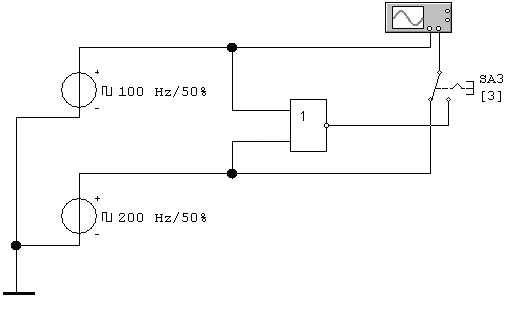
\includegraphics[]{schematics/05-02-NOR.png}
			\caption{Принципова схема для перевірки динамічного режиму роботи логічного елемента «АБО—НЕ»}
			\label{fig:NOR-dynamic-mode-schematic}
			\end{figure}
			
			Отримали осцилограму вхідних сигналів. Встановлюємо перемикач \schel{SA3} у праве положення і отримаємо осцилограму вихідного сигналу.
			
			За отриманими даними будуємо часову діаграму логічного елемента «І». Побудована діаграма зображена на рисунку~\ref{fig:NOR-time-diagram}.
			
			\begin{figure}[!htbp]
			\centering
				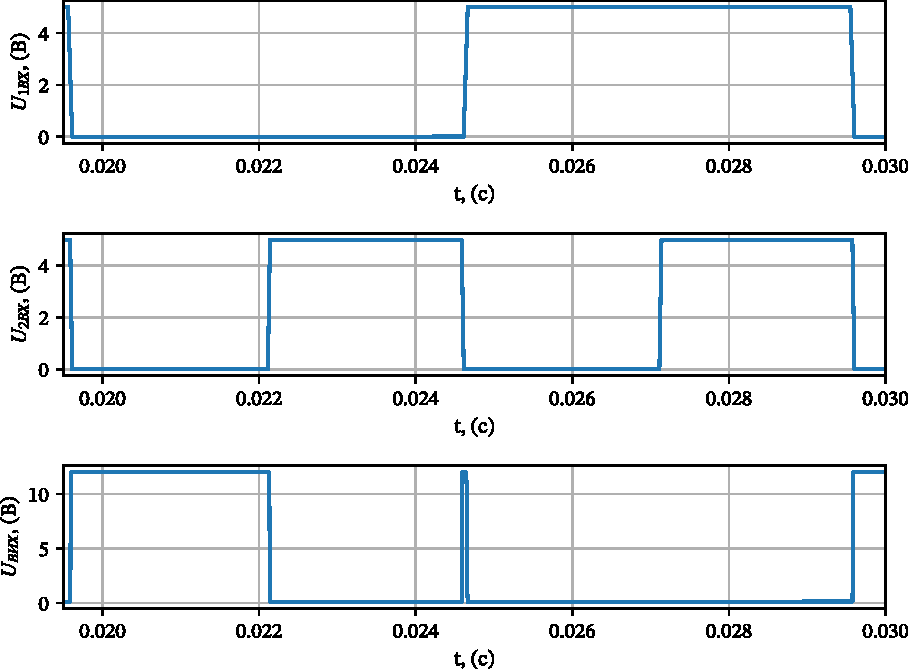
\includegraphics[width=\textwidth]{plots/03-pdf/05-NOR-time-diagram-edited.pdf}
			\caption{Часова діаграма логічного елемента «АБО—НЕ»}
			\label{fig:NOR-time-diagram}
			\end{figure}
			
			\begin{table}[!htbp]
			\centering
				\begin{tabular}{ccr}
					\toprule
						$x_1$ & $x_2$ & $f(x_1, x_2)$\\
					\midrule
						0     & 0     & 1\\
						0     & 1     & 0\\
						1     & 0     & 0\\
						1     & 1     & 0\\
					\bottomrule
				\end{tabular}
			\caption{Таблиця істинності логічного елемента «АБО—НЕ»}
			\label{fig:NOR-truth-table}
			\end{table}
			
	\section{Висновки}
		Під час виконання лабораторної роботи ми практично перевірили роботу логічних елементів різних функціонально повних наборів. Освоїли методику визначення основних характеристик логічних елементів та визначили їх. Вивчили закони функціонування логічних елементів «НЕ», «І», «АБО», «АБО—НЕ», «І—НЕ». Вивчили методику визначення часових параметрів логічних елементів.
		
\end{document}
